\documentclass[11pt,openright,final]{unsa}
\title{Framework de explicabilidad agnóstica al modelo para la predicción de series temporales financieras}
\author{Rushell Vanessa Zavalaga Orozco}%
\advisor{Juan Carlos Gutiérrez Cáceres}{Asesor}%
% PENDIENTE: nombres reales del jurado. Reemplazar los placeholders entre
% corchetes antes de compilar la versión final.
\examinerone{[Nombre del presidente del jurado]}{Presidente}%
\examinertwo{[Nombre del secretario del jurado]}{Secretario}%
\examinerthree{[Nombre del integrante del jurado]}{Integrante}%

\date{\today}
\dedicate{A mi familia, por su apoyo constante en cada etapa de este
camino; y a mis profesores, por la formación recibida a lo largo de
la carrera.}

\begin{document}%%%%%%%%-------------------------------------------------------
\makeFirstCover
\makeSecondCover %
\begin{frontmatter}
\approved{\tres}% {\tres} si son 3 jurados, {\cuatro} si hay un jurado adicional
\dedicatory
\begin{singlespace}
\tableofcontents \listoftables \pagebreak
\end{singlespace}
\myAcknowledgements{Agradecimientos}%
\myResumen{Resumen}%
\myAbstrac{Abstract}%
\end{frontmatter}%
\pagestyle{fancyplain}
\chapter{Introducción}
\hrule \bigskip \vspace*{1cm}
%------------------------------------------------------------------------

\label{sec:introduccion}

Este capítulo presenta el problema abordado por la tesis y la propuesta desarrollada para resolverlo. La Sección~\ref{sec:contexto} sitúa el problema en el contexto de la gestión de riesgos financieros, y la Sección~\ref{sec:motivacion} expone por qué la falta de explicabilidad de los modelos de aprendizaje automático es un problema práctico y regulatorio. La Sección~\ref{sec:planteamiento_problema} formaliza la brecha específica que ningún método previo cubre. La Sección~\ref{sec:justificacion} justifica la propuesta frente a las limitaciones de los trabajos más cercanos. Las Secciones~\ref{sec:objetivo_general} y \ref{sec:objetivos_especificos} presentan el objetivo general, con el flujo del framework, y los objetivos específicos que guían el trabajo. Finalmente, la Sección~\ref{sec:organizacion_tesis} describe la organización del resto del documento.

\section{Contexto}
\label{sec:contexto}

La predicción de series temporales financieras, como el precio de cierre diario de un índice bursátil, se usa en la práctica para decidir directamente sobre un portafolio, cuándo comprar, mantener o vender una posición, o cuánto capital asignar a un activo frente a otro \cite{arsenault2025}. El riesgo financiero relevante para esta tesis es exactamente esa traducción, la pérdida de valor que se materializa sobre el portafolio cuando la decisión se apoyó en una predicción que resultó incorrecta. Estas consecuencias no son solo teóricas. Cohen et al.\ \cite{cohen2023blackbox} documentan que la opacidad de los modelos de aprendizaje automático usados para generar esas predicciones agrega una segunda capa a ese riesgo, el \emph{riesgo de modelo} (\emph{model risk}), definido por el propio SR~11-7 \cite{sr117} como el riesgo de consecuencias adversas derivadas de decisiones basadas en resultados de modelos incorrectos o mal utilizados. A diferencia del riesgo de que el precio se mueva en contra, que existe incluso con un modelo perfectamente entendido, el riesgo de modelo existe porque nadie puede validar si el modelo aprendió una relación económica real o una coincidencia sin significado presente en los datos de entrenamiento, hasta que la decisión ya se tomó. Esta tesis se ubica específicamente en el riesgo de modelo, no en el riesgo de que el mercado se mueva en contra. Este riesgo no es hipotético dentro del propio trabajo, la consistencia entre modelos que se mide como criterio de validación (Sección~\ref{sec:estrategia_validacion}) resulta sistemáticamente menor durante el régimen bajista de 2022 que durante el régimen alcista de 2023 y 2024 (Capítulo~5), es decir, el desacuerdo entre modelos sobre qué variables importan aumenta justo en el escenario donde una decisión errónea es más costosa para una institución.

\section{Motivación}
\label{sec:motivacion}

En los últimos años, los modelos de aprendizaje profundo han reducido el error de predicción sobre este tipo de datos frente a métodos estadísticos clásicos \cite{bhandari2022, abdulquadir2023}. Sin embargo, estos modelos no explican por qué llegan a cada resultado, y esa falta de explicación ya tiene consecuencias regulatorias concretas. El SR 11-7 de la Reserva Federal estadounidense \cite{sr117} obliga a los bancos a demostrar que entienden las capacidades y los límites de cada modelo antes de usarlo. El Reglamento de Inteligencia Artificial de la Unión Europea \cite{euaiact2024} exige, para ciertos usos financieros como la evaluación crediticia, que el modelo sea lo bastante transparente para que quien lo usa pueda interpretar sus resultados. Pese a estas exigencias, Sovrano et al.\ \cite{sovrano2026} muestran que los métodos de explicabilidad actuales todavía no las cumplen de forma sistemática.

Para abordar esta opacidad, el campo de la Inteligencia Artificial Explicable (XAI) agrupa métodos que permiten identificar qué factores influyeron en una predicción. Estos métodos se organizan en familias según su mecanismo. Los basados en gradientes, como DeepLIFT \cite{shrikumar2017}, requieren acceso a la estructura interna del modelo. Los basados en atención dependen de la arquitectura utilizada, y su equivalencia con una explicación es discutida \cite{jain2019}. Los basados en perturbación, como SHAP y LIME, son agnósticos al modelo porque generan explicaciones observando cómo cambia la salida al modificar partes de la entrada \cite{arsenault2025}. Esta capacidad no depende de ninguna propiedad especial del modelo, solo requiere poder consultarlo como una función que recibe una entrada y devuelve una predicción, sin inspeccionar pesos ni gradientes, por lo que el mismo mecanismo se aplica sin modificación tanto a una red neuronal como a un modelo de ensamble o a un modelo estadístico clásico. El costo de esa generalidad es que, a diferencia de un método de gradiente que obtiene la sensibilidad local en una sola operación analítica, un método de perturbación necesita consultar el modelo una vez por cada elemento de la entrada cuya influencia quiere medir. No obstante, estos últimos asumen, en su formulación habitual, que las variables de entrada son independientes entre sí \cite{lundberg2017, ribeiro2016}. Al aplicarse sobre series temporales, tratan cada paso de tiempo como una variable aislada, ignorando que las observaciones forman una secuencia con dependencias estructurales \cite{tonekaboni2020, huang2025}.

Construir un framework de explicabilidad para este dominio conlleva responsabilidades éticas concretas, no solo declarativas. Un modelo entrenado sobre datos financieros históricos hereda los sesgos de ese historial, un régimen de mercado específico \cite{angtimmermann2012}, la composición cambiante del índice, la autocorrelación trivial del precio \cite{fama1970, meese1983}, y una explicación poco fiel puede ocultar esos sesgos en vez de exponerlos \cite{rudin2019}. Por esta razón, este trabajo reporta también los resultados que no favorecen a la propuesta, que ningún modelo entrenado supera el baseline de persistencia ingenua y que la consideración específica investigada para Random Forest (Sección~\ref{sec:leaf_reference_propuesta}) no confirmó la hipótesis inicial, en vez de omitirlos. Además, al no requerir gradientes ni una optimización costosa por instancia, el framework reduce la barrera computacional y de infraestructura para auditar modelos financieros, una consideración de acceso equitativo relevante para instituciones o reguladores sin la capacidad de cómputo que exigen métodos como Shapley Value Sampling o las máscaras aprendidas por gradiente, y reduce a la vez el costo energético asociado a esa auditoría.

\section{Planteamiento del Problema}
\label{sec:planteamiento_problema}

El problema que aborda esta tesis puede formularse como un problema de cómputo con dos requisitos que ningún método previo satisface a la vez. Primero, que el mecanismo de explicación funcione sobre arquitecturas de naturaleza computacional distinta sin acceder a su implementación interna. Segundo, que ese mecanismo tenga un costo fijo por instancia, evaluable en una sola pasada, sin resolver una optimización propia cada vez que se explica una predicción.

Los métodos con acceso a la estructura interna del modelo logran coherencia temporal en la atribución pero quedan acoplados a una arquitectura específica, los pesos de atención de un Transformer no tienen equivalente en un modelo de ensamble como Random Forest \cite{arsenault2025}. Los métodos de perturbación agnósticos sí funcionan sobre cualquier modelo, pero generan perturbaciones que rompen la dependencia estructural entre observaciones consecutivas \cite{tonekaboni2020, huang2025}.

Existen métodos que respetan el orden temporal, como las máscaras dinámicas de Crabbé y Van Der Schaar \cite{crabbe2021}, pero ajustan la perturbación resolviendo, para cada instancia, un problema de optimización no convexo mediante descenso de gradiente, lo que además de un costo computacional considerable les impide operar sobre modelos no diferenciables como Random Forest. Dos extensiones directas de este método, publicadas en ICML \cite{enguehard2023} e ICLR \cite{liu2024contralsp}, corrigen la calidad de la perturbación pero mantienen la misma dependencia del gradiente. Cinco años después de la propuesta original, ningún método de esta línea de trabajo funciona sin gradientes, y ninguno se ha validado sobre series financieras pese a mencionarlas como motivación. Random Forest es, en este sentido, el caso concreto que hace tangible el problema, sigue siendo estado del arte en datos tabulares \cite{grinsztajn2022}, y es precisamente el tipo de modelo que esta línea de trabajo excluye por diseño.

El costo fijo por instancia que exige el segundo requisito no es una meta de eficiencia aislada, depende directamente de cómo se resuelva el primer requisito. Las máscaras dinámicas de Crabbé y Van Der Schaar \cite{crabbe2021} son intrínsecamente secuenciales, cada paso del descenso de gradiente parte del resultado del paso anterior, así que su costo por instancia crece con el número de iteraciones que necesite converger y no puede reducirse agrupando esas iteraciones en una sola operación. El mecanismo de perturbación agnóstico que exige el primer requisito tiene, en cambio, una propiedad distinta, perturbar la celda $(t,v)$ para medir su influencia no depende del resultado de perturbar ninguna otra celda $(t',v')$. Al no existir esa dependencia entre perturbaciones, todas pueden evaluarse en un único conjunto de consultas al modelo procesado de una vez, en vez de una secuencia de pasos donde cada uno espera al anterior. Por esta razón el framework propuesto en esta tesis no necesita diseñarse ni optimizarse aparte para ejecutar en paralelo, la independencia entre perturbaciones que exige la agnosticidad hace que la versión de una sola pasada sea, al mismo tiempo, la versión paralela.

\subsection{Estrategia de validación}
\label{sec:estrategia_validacion}

La independencia entre perturbaciones descrita en el párrafo anterior también define cómo se valida la propuesta a lo largo de la tesis, en dos etapas con una naturaleza distinta cada una.

La primera etapa usa datos sintéticos generados por una función matemática definida por la propia investigadora, no aprendida ni etiquetada externamente. La función se construye de forma que su salida dependa matemáticamente solo de un subconjunto pequeño y conocido de celdas $(t,v)$ de la ventana de entrada, por ejemplo $f(X) = \sum_{(t,v) \in A} x_{t,v}^2$, donde $A$ es ese subconjunto elegido de antemano. El resto de las celdas de $X$ no aparece en la fórmula, así que no puede influir en la salida. Como la función es propia, el conjunto $A$ de celdas relevantes se conoce con certeza, y sirve como ground truth contra el cual comparar la matriz de importancia que produce el framework, esa comparación es la que permite calcular métricas de precisión y cobertura como AUP y AUR (Capítulo~5). Esta es la misma estrategia que usó DynaMask con sus propios datasets sintéticos \cite{crabbe2021}, la diferencia con esta tesis está en el dominio de la función construida, no en el mecanismo de validación.

La segunda etapa usa el S\&P~500 real, donde no existe una función conocida que genere el precio del día siguiente y, por lo tanto, tampoco existe un conjunto $A$ verdadero contra el cual comparar. Al no haber ground truth, la validación deja de medir precisión directa y pasa a depender de señales indirectas de que la explicación refleja el comportamiento real del modelo y no un artefacto del método \cite{adebayo2018}, que las atribuciones sean estadísticamente distintas de una asignación aleatoria, que sean consistentes entre modelos de mecanismo similar y menos consistentes entre modelos de mecanismo distinto (objetivo específico 4), y que se mantengan estables frente a variaciones del propio procedimiento, el orden temporal de la perturbación, el vector de referencia usado y el régimen de mercado evaluado. Esta segunda etapa es la que corresponde específicamente al dominio y al tema de estudio de esta tesis, series temporales financieras sin ground truth disponible, y es donde el aporte de validación es más propio del trabajo.

\section{Justificación}
\label{sec:justificacion}

Los trabajos relacionados descritos en los párrafos anteriores resuelven, cada uno, solo uno de los dos requisitos planteados en el Planteamiento del Problema (Sección~\ref{sec:planteamiento_problema}), nunca ambos a la vez. Los métodos de perturbación agnósticos como SHAP y LIME satisfacen el primer requisito, funcionan sobre cualquier arquitectura sin acceder a su interior, pero no el segundo, porque al tratar cada paso de tiempo como una variable independiente rompen el orden temporal de la serie \cite{tonekaboni2020, huang2025}. Las máscaras dinámicas de Crabbé y Van Der Schaar \cite{crabbe2021} y sus extensiones en ICML \cite{enguehard2023} e ICLR \cite{liu2024contralsp} satisfacen el segundo requisito en cuanto a coherencia temporal, pero no el primero, porque su optimización por descenso de gradiente las ata a modelos diferenciables y excluye por diseño a modelos no diferenciables como Random Forest. Ninguno de los dos grupos ha sido validado además sobre series financieras pese a mencionarlas como motivación.

El motor de perturbaciones temporales propuesto en esta tesis (Capítulo~4) se diseña precisamente para cerrar esa brecha compartiendo la propiedad que las máscaras dinámicas no tienen y que los métodos agnósticos clásicos tampoco tienen en su formulación original. Perturba una sola celda $(t,v)$ a la vez, dejando el resto de la ventana exactamente en su valor y posición observados, lo que preserva el orden temporal sin necesidad de gradientes ni de una optimización propia por instancia. Esta decisión de diseño es la que permite explicar bajo el mismo mecanismo a los tres modelos entrenados en esta tesis, LSTM, Transformer y Random Forest, y es la que se somete a verificación empírica en el Capítulo~5, tanto contra un ground truth sintético conocido como sobre el S\&P~500 real.

\section{Objetivo General}
\label{sec:objetivo_general}

Desarrollar un framework de explicabilidad temporal agnóstico al modelo para la predicción de series temporales financieras, que atribuya importancia por variable y paso de tiempo sin depender de la estructura interna del modelo explicado ni requerir acceso a sus gradientes, y cuyo costo de cómputo por instancia sea fijo y evaluable en una sola pasada paralela, sin resolver una optimización propia para cada predicción explicada.

El flujo completo del framework se resume en la Figura~\ref{fig:pipeline} y se detalla en el Capítulo~4. Los datos de entrada y su preparación, en azul, alimentan a un modelo predictivo, en verde, que se conecta con el motor de perturbación mediante una interfaz uniforme de predicción. El motor, en naranja, es la contribución principal y produce la matriz de importancia temporal.

\begin{figure}[ht]
\centering
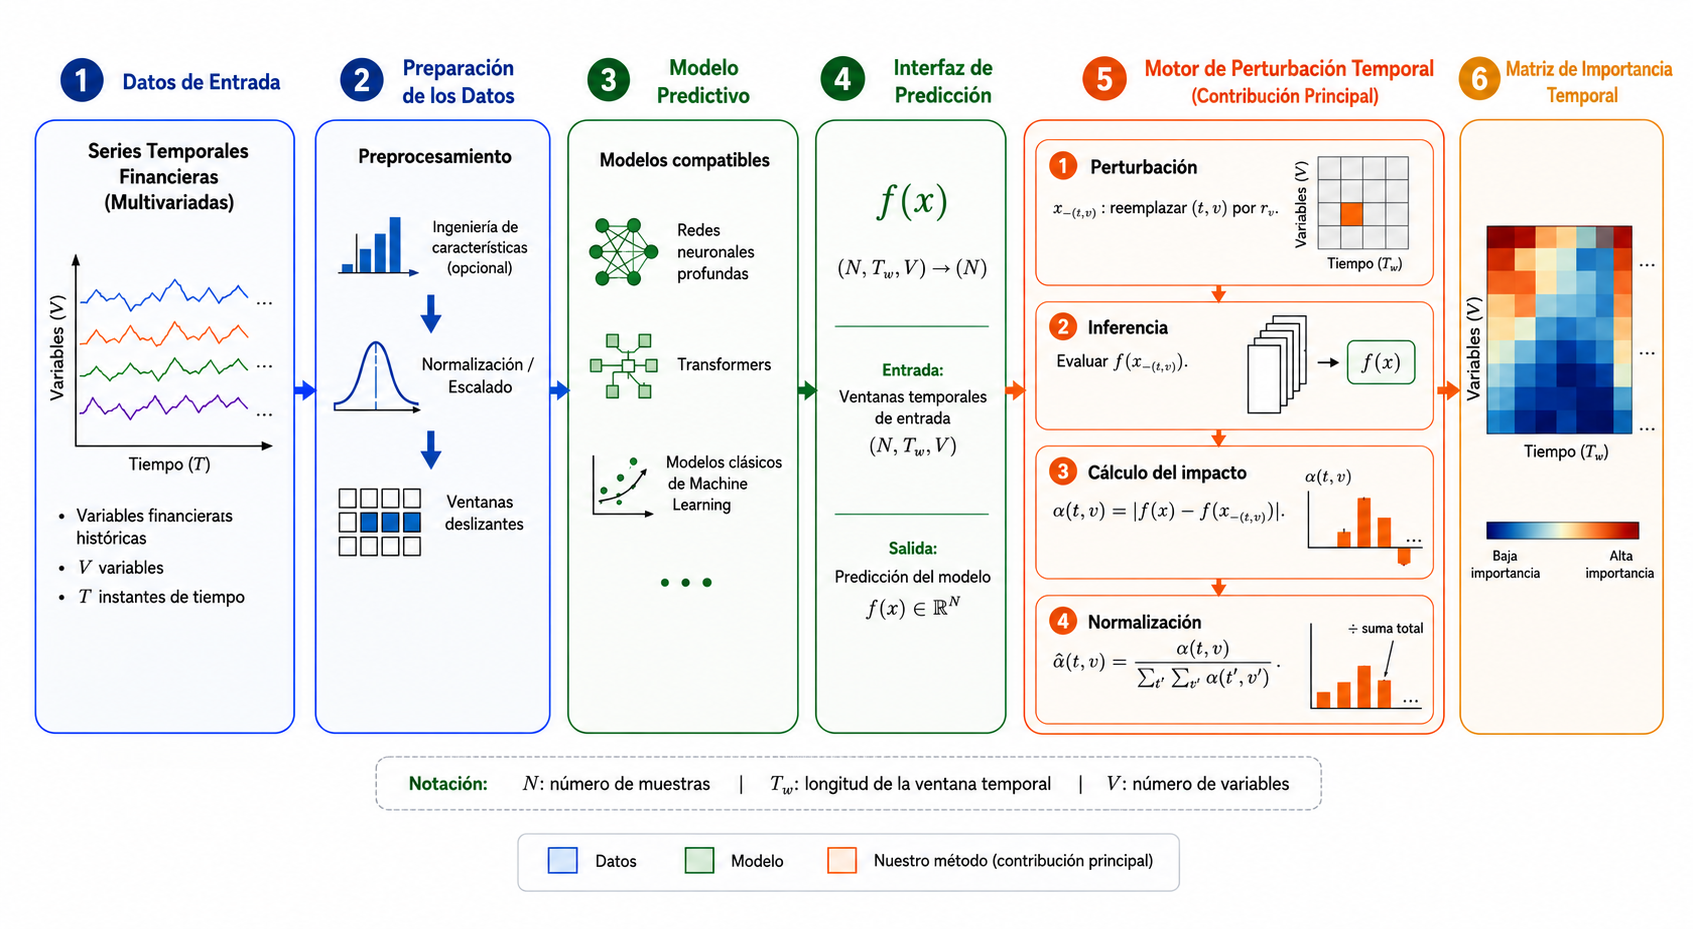
\includegraphics[width=\textwidth]{Graficos/PIPELINE.png}
\caption{Pipeline del framework en seis etapas. (1)~Datos de entrada, series temporales financieras multivariadas. (2)~Preparación de los datos, con ingeniería de características, normalización y ventanas deslizantes. (3)~Modelo predictivo, que puede ser una red neuronal, un Transformer o un modelo clásico de aprendizaje automático. (4)~Interfaz de predicción, que recibe ventanas de forma $(N,T,V)$ y devuelve $N$ predicciones. (5)~Motor de perturbación temporal, con perturbación de una celda, inferencia, cálculo del impacto y normalización. (6)~Matriz de importancia temporal $\hat{\alpha}$. En la figura, $T_w$ denota la longitud $T$ de la ventana.}
\label{fig:pipeline}
\end{figure}

\section{Objetivos Específicos}
\label{sec:objetivos_especificos}

\begin{enumerate}
    \item Diseñar una interfaz uniforme de predicción, mediante un patrón adaptador de dos niveles, que desacople el motor de perturbaciones de la estructura interna de cualquier modelo.
    \item Formular un motor de perturbaciones temporales que atribuya importancia a nivel de celda $(t,v)$, preservando el orden y la coherencia temporal del resto de la ventana, y cuyas perturbaciones sean independientes entre sí para poder evaluarse en un único batch paralelo en vez de una secuencia de pasos de optimización.
    \item Entrenar modelos de distinta naturaleza computacional (LSTM, Transformer, Random Forest) sobre el S\&P~500 como banco de pruebas del framework.
    \item Verificar que las explicaciones generadas reflejan el comportamiento específico de cada modelo, y no son independientes del modelo explicado ni artefacto del procedimiento, esperando mayor consistencia entre modelos de mecanismo similar (LSTM y Transformer) que frente a un modelo de mecanismo distinto (Random Forest). Esta expectativa de divergencia parcial, no de igualdad total, sigue el criterio de Adebayo et al.\ \cite{adebayo2018}, quienes muestran que un método de explicación que produce el mismo resultado sin importar el modelo explicado, incluso con sus pesos aleatorizados, no está reflejando ese modelo sino reproduciendo un artefacto propio del método. Que la atribución cambie con la arquitectura, en una proporción coherente con cuánto se parece su mecanismo interno al de otras arquitecturas evaluadas, es la evidencia a favor del framework, no una inconsistencia a corregir.
    \item Evaluar el framework frente al estado del arte agnóstico en precisión de identificación, consistencia entre modelos y velocidad de cómputo.
    \item Investigar si existe una consideración anclada en la estructura particular de Random Forest que reduzca su mayor sensibilidad observada al vector de referencia, y documentar el resultado con la misma rigurosidad tanto si confirma como si descarta la hipótesis.
\end{enumerate}

\section{Organización de la tesis}
\label{sec:organizacion_tesis}

El Capítulo~2 presenta el marco teórico, que parte de las series temporales financieras y los modelos que se entrenan sobre ellas, define la interpretabilidad y la explicabilidad, y formaliza la explicabilidad post-hoc, el agnosticismo al modelo, los métodos de perturbación, la explicabilidad temporal y los criterios de evaluación de una explicación. El Capítulo~3 revisa los trabajos relacionados de los últimos cinco años, organizados en tres ejes, los métodos de perturbación agnósticos que incorporan de algún modo la dimensión temporal, los frameworks explícitamente diseñados para ser temporalmente conscientes y agnósticos a la vez, incluyendo el linaje directo de DynaMask, y los explicadores aprendidos con objetivos de cuello de botella de información. El Capítulo~4 describe la propuesta, la interfaz uniforme de predicción, el motor de perturbaciones temporales, los tres modelos entrenados, y la investigación de una consideración específica para Random Forest. El Capítulo~5 presenta los resultados experimentales, desempeño predictivo, validación con ground truth sintético, verificación de agnosticismo sobre el S\&P~500, pruebas de robustez, y comparación con el estado del arte. El Capítulo~6 cierra con las conclusiones, las limitaciones del trabajo y el trabajo futuro planificado.

\chapter{Marco Teórico}
\hrule \bigskip \vspace*{1cm}
%------------------------------------------------------------------------
\label{chap:marco_teorico}

\section{Consideraciones iniciales}

Este capítulo presenta los conceptos sobre los que se construye la propuesta del Capítulo~4. El orden es deliberado y va de lo general a lo específico. Parte del objeto que se quiere explicar, las series temporales financieras, con las propiedades estadísticas que condicionan cualquier modelo y cualquier explicación. Continúa con los modelos que se entrenan sobre esas series, de naturaleza computacional distinta, porque esa diferencia determina qué métodos de explicación pueden aplicarse a cada uno. Luego define qué significa interpretar y explicar un modelo, y por qué la explicación es una necesidad en el sector financiero. Después presenta las propiedades que se exigen a un método de explicación, que sea post-hoc y agnóstico al modelo, y las familias de métodos de atribución, de las cuales se deriva la perturbación. Formaliza a continuación la explicabilidad temporal, que es el problema específico que resuelve este trabajo, y describe las líneas más recientes del área, las máscaras aprendidas, las explicaciones contrafactuales y el cuello de botella de información. Cierra con los criterios que se emplean para evaluar si una explicación es confiable.

\section{Series temporales financieras}
\label{sec:mt_series}

\subsection{Definición y formulación como ventana de entrada}
\label{sec:mt_ventana}

Una serie temporal es una secuencia de observaciones ordenadas en el tiempo, y es multivariada cuando cada instante reúne varias variables medidas a la vez \cite{tsay2010}. En finanzas, la observación de un día puede contener el precio de apertura, el máximo, el mínimo, el cierre, el volumen negociado y otras cantidades derivadas de ellas. La predicción de series temporales consiste en estimar el valor futuro de una variable de interés a partir de su historia, y el aprendizaje profundo se ha consolidado como una de las familias de métodos más usadas para esta tarea \cite{lim2021}. En el ámbito financiero, Sezer et al.\ \cite{sezer2020} revisan la literatura de 2005 a 2019 sobre el uso de aprendizaje profundo en el pronóstico de series financieras, y Kumbure et al.\ \cite{kumbure2022} hacen lo propio para las técnicas de aprendizaje automático y los datos de entrada empleados en la predicción de mercados bursátiles.

Los modelos de aprendizaje automático no reciben la serie completa, reciben una ventana de longitud fija formada por los últimos $T$ pasos de tiempo \cite{lim2021}. Dado un instante $\tau$, la entrada es la matriz
\begin{equation}
    x = \begin{pmatrix} x_{\tau-T+1,1} & \cdots & x_{\tau-T+1,V} \\ \vdots & \ddots & \vdots \\ x_{\tau,1} & \cdots & x_{\tau,V} \end{pmatrix} \in \mathbb{R}^{T \times V},
    \label{eq:ventana}
\end{equation}
donde $V$ es el número de variables. Un modelo predictivo es una función $f\colon \mathbb{R}^{T \times V} \rightarrow \mathbb{R}$ que asigna a cada ventana una predicción $\hat{y} = f(x)$ del valor de la variable objetivo en el instante siguiente. Cada celda $(t,v)$ de la ventana corresponde a una variable en un paso de tiempo, y es la unidad sobre la que esta tesis atribuye importancia.

\subsection{Retornos y propiedades estadísticas de las series financieras}
\label{sec:mt_retornos}

Los precios no se modelan directamente, se modelan sus retornos. El retorno logarítmico entre dos instantes consecutivos se define como $r_{\tau+1} = \ln(P_{\tau+1}/P_{\tau})$, donde $P$ es el precio de cierre, y se prefiere sobre el precio porque es aditivo en el tiempo y su media es aproximadamente estable \cite{tsay2010}. El precio, en cambio, crece con el tiempo y produce valores fuera del rango observado durante el entrenamiento.

Cont \cite{cont2001} recopila un conjunto de regularidades estadísticas que se observan de forma consistente en retornos de distintos activos, mercados y periodos, y que denomina hechos estilizados. Tres de ellas son relevantes para esta tesis. La primera es la ausencia de autocorrelación lineal significativa en los retornos, lo que significa que el retorno de hoy casi no se puede predecir linealmente a partir del de ayer. La segunda es la presencia de colas pesadas en la distribución de los retornos, es decir, que los movimientos extremos son más frecuentes de lo que predice una distribución normal. La tercera es el agrupamiento de volatilidad, la tendencia de los periodos de alta variación a concentrarse juntos en el tiempo. Estas propiedades hacen que el retorno sea una variable objetivo difícil de predecir y que su relación con las variables de entrada cambie según el momento.

\subsection{Eficiencia de mercado y el baseline de persistencia}
\label{sec:mt_eficiencia}

La hipótesis de mercado eficiente, formalizada por Fama \cite{fama1970}, sostiene que los precios reflejan la información disponible. En su forma débil, esa información es la historia pasada de los precios, de modo que ningún modelo que solo use precios y volúmenes pasados debería obtener una ventaja sistemática. Una consecuencia práctica es que la mejor predicción del valor siguiente de un precio es, en primera aproximación, el último valor observado, que se conoce como baseline de persistencia o paseo aleatorio.

Este criterio no es solo teórico. Meese y Rogoff \cite{meese1983} mostraron, en el mercado de divisas, que los modelos estructurales de tipo de cambio no superaban fuera de muestra a un paseo aleatorio, y desde entonces la comparación con ese baseline es un estándar para juzgar modelos de pronóstico financiero. Por el lado del aprendizaje automático, Gu et al.\ \cite{gu2020} comparan distintos métodos para predecir primas de riesgo de activos y encuentran que los árboles de decisión y las redes neuronales son los de mejor desempeño, lo que atribuyen a su capacidad de capturar interacciones no lineales entre los predictores. Esto justifica el uso de ambas familias de modelos, pero no elimina la necesidad de compararlas con un baseline simple. Para la explicabilidad esto tiene una consecuencia metodológica. Un modelo que no supera al baseline de persistencia no aporta información propia sobre la serie, y explicarlo equivale a explicar un artefacto de la autocorrelación trivial del precio, por lo que este trabajo reporta ese baseline junto con los modelos que explica.

\subsection{No estacionariedad y regímenes de mercado}
\label{sec:mt_regimenes}

Las series financieras no mantienen sus propiedades estadísticas en el tiempo. Hamilton \cite{hamilton1989} propuso modelar series no estacionarias como procesos que alternan entre distintos regímenes, cada uno con parámetros propios, y Ang y Timmermann \cite{angtimmermann2012} revisan la evidencia de que los mercados financieros presentan cambios de régimen persistentes en la media, la volatilidad y las correlaciones de los retornos. En la práctica, esto se traduce en tramos alcistas de baja volatilidad que alternan con tramos bajistas de alta volatilidad.

Esta no estacionariedad tiene dos consecuencias para la explicabilidad. Primero, una explicación válida en un régimen puede dejar de serlo en otro, por lo que debe evaluarse por régimen y no solo como promedio sobre todo el periodo. Segundo, los supuestos de suavidad o estacionariedad local, que varios métodos temporales asumen para construir sus perturbaciones, se violan justo en los momentos de mayor interés para la gestión del riesgo.

\subsection{Variables de entrada, indicadores técnicos y ventanas deslizantes}
\label{sec:mt_variables}

Además de los precios y el volumen, la literatura de predicción bursátil utiliza de forma habitual indicadores técnicos, cantidades derivadas del precio y del volumen que resumen tendencia, momentum o volatilidad \cite{kumbure2022}. En esta tesis se derivan diez a partir de las cinco series base. Las medias móviles simples de $n$ días, $\mathrm{SMA}_n(\tau)=\frac{1}{n}\sum_{i=0}^{n-1}P_{\tau-i}$, resumen la tendencia. El MACD es la diferencia entre dos medias móviles exponenciales de periodos distintos, y su señal es una media móvil exponencial del propio MACD. El índice de fuerza relativa (RSI) compara la magnitud de las subidas y las bajadas recientes. El ancho de las bandas de Bollinger mide la dispersión del precio alrededor de su media móvil. El rango verdadero promedio (ATR) mide la volatilidad a partir de los rangos diarios, el retorno logarítmico es el definido en la Sección~\ref{sec:mt_retornos} y el volumen relativo compara el volumen del día con su promedio reciente. Con las cinco variables base resultan $V=15$ variables por paso de tiempo.

Las ventanas se construyen deslizando una ventana de longitud $T$ sobre la serie y emparejando cada una con el valor objetivo del instante siguiente. La partición de los datos en desarrollo y prueba debe respetar el orden temporal, y cualquier transformación que se ajuste con los datos, como una normalización, debe ajustarse solo con el periodo de desarrollo para no filtrar información del futuro hacia el pasado.

\section{Modelos predictivos de distinta naturaleza computacional}
\label{sec:mt_modelos}

Los modelos que se entrenan sobre estas ventanas difieren en cómo las procesan, y esa diferencia es la razón por la que un método de explicación debe ser verificado en más de una arquitectura.

\subsection{Redes de memoria larga (LSTM)}

Una red LSTM \cite{hochreiter1997} es una red neuronal recurrente que procesa la ventana paso a paso y resume el pasado en un estado interno. Incorpora compuertas que regulan qué información se escribe, se conserva y se descarta de ese estado, un diseño que busca conservar dependencias de largo plazo que las redes recurrentes simples pierden durante el entrenamiento. Es un modelo diferenciable, de modo que el gradiente de su salida respecto de la entrada puede calcularse.

\subsection{Transformer}

El Transformer \cite{vaswani2017} reemplaza la recurrencia por el mecanismo de autoatención, en el que cada paso de la secuencia se compara con todos los demás para decidir cuánto debe pesar cada uno en su representación. Su aplicación a series temporales ha dado lugar a una familia amplia de variantes, revisada por Wen et al.\ \cite{wen2023}. Como la autoatención no distingue por sí sola el orden de los pasos, se le añade una codificación posicional. Para producir una única predicción a partir de la secuencia, una opción es agregar los pasos con pesos aprendidos mediante una capa de atención, en vez de usar solo el último paso, que es la elección que se usa en este trabajo. Al igual que la LSTM, es diferenciable.

\subsection{Bosques aleatorios (Random Forest)}

Un bosque aleatorio \cite{breiman2001} es un conjunto de árboles de decisión entrenados cada uno sobre una muestra bootstrap de los datos y con una selección aleatoria de atributos en cada división. En regresión, su predicción es el promedio de las predicciones de los árboles. No tiene noción de secuencia, de modo que recibe la ventana aplanada como un vector de $T \cdot V$ atributos, y cada celda es para el modelo un atributo tabular más. No es diferenciable, porque sus predicciones son constantes por tramos. Una consecuencia directa de su definición es que cada hoja predice el promedio de los valores objetivo vistos en el entrenamiento, por lo que la salida del bosque queda dentro del rango de esos valores y no puede extrapolar más allá de él. Esto es relevante para series financieras con tendencia, y es una de las razones para entrenar sobre retornos y no sobre precios. A pesar de ello, los modelos basados en árboles siguen siendo competitivos frente al aprendizaje profundo en datos tabulares de tamaño mediano \cite{grinsztajn2022}.

\subsection{Diferenciabilidad y acceso al modelo}

La Tabla~\ref{tab:mt_modelos} resume las propiedades de los tres modelos que importan para la explicabilidad. Que los dos primeros sean diferenciables y el tercero no decide qué métodos de atribución pueden aplicarse a cada uno, un punto que se desarrolla en la Sección~\ref{sec:mt_familias}.

\begin{table}[h!]
\centering
\small
\renewcommand{\arraystretch}{1.25}
\begin{tabular}{|>{\raggedright\arraybackslash}p{2.9cm}|>{\raggedright\arraybackslash}p{4.3cm}|>{\centering\arraybackslash}p{2.6cm}|>{\raggedright\arraybackslash}p{2.8cm}|}
\hline
\textbf{Modelo} & \textbf{Cómo procesa la ventana} & \textbf{Diferenciable} & \textbf{Entrada} \\ \hline
LSTM & Recurrente, paso a paso & Sí & Secuencia $(T,V)$ \\ \hline
Transformer & Autoatención entre todos los pasos & Sí & Secuencia $(T,V)$ \\ \hline
Random Forest & Promedio de árboles, sin noción de secuencia & No & Vector de $T\cdot V$ atributos \\ \hline
\end{tabular}
\caption{Modelos empleados y propiedades relevantes para la explicabilidad (referencias en la Sección~\ref{sec:mt_modelos}).}
\label{tab:mt_modelos}
\end{table}

\section{Interpretabilidad y explicabilidad}
\label{sec:mt_interpretabilidad}

\subsection{Definiciones}

Los términos interpretabilidad y explicabilidad suelen usarse como sinónimos, pero designan ideas cercanas y distintas. Doshi-Velez y Kim \cite{doshivelez2017} definen la interpretabilidad como la capacidad de explicar o presentar el comportamiento de un modelo en términos comprensibles para una persona. Barredo Arrieta et al.\ \cite{arrieta2020} distinguen entre modelos transparentes, que son comprensibles por su propia estructura, y la explicabilidad como el conjunto de acciones o procedimientos que produce un modelo para dejar claros los motivos de su funcionamiento. Lipton \cite{lipton2018} advierte que la interpretabilidad no es una propiedad única y bien definida sino un conjunto de objetivos distintos, como la confianza, la auditoría o la identificación de causas, y que por eso una explicación debe evaluarse siempre respecto de un propósito.

\subsection{Taxonomía de los métodos}

Guidotti et al.\ \cite{guidotti2018} organizan los métodos de explicación según el problema que resuelven. Distinguen explicar el modelo completo, explicar el resultado de una instancia particular e inspeccionar el comportamiento de una caja negra. Esto da lugar a dos ejes. El primero separa las explicaciones \emph{locales}, que justifican una predicción individual, de las \emph{globales}, que describen el comportamiento general del modelo. Esta tesis trabaja con explicaciones locales, una matriz de importancia por cada ventana explicada. El segundo eje separa los modelos interpretables por diseño, como un árbol de decisión individual o una regresión lineal, de los métodos que explican modelos ya construidos, que son los llamados métodos post-hoc.

Rudin \cite{rudin2019} sostiene que para decisiones de alto riesgo es preferible usar modelos interpretables por diseño en lugar de explicar a posteriori una caja negra, entre otras razones porque una explicación post-hoc no es completamente fiel al modelo que explica. Este argumento no invalida el enfoque de esta tesis, pero sí fija una exigencia, que la fidelidad de la explicación debe medirse y no darse por supuesta, tema que se desarrolla en la Sección~\ref{sec:mt_evaluacion}.

\subsection{La explicabilidad en el sector financiero}

La necesidad de explicar los modelos financieros tiene un origen regulatorio. La guía SR~11-7 de la Reserva Federal de los Estados Unidos \cite{sr117} exige a los bancos comprender las capacidades y los límites de un modelo antes de usarlo, y define el riesgo de modelo como el riesgo de consecuencias adversas derivadas de decisiones basadas en resultados de modelos incorrectos o mal utilizados. Cohen et al.\ \cite{cohen2023blackbox} documentan que la opacidad de los modelos de aprendizaje automático agrega una capa adicional a ese riesgo. El Reglamento de Inteligencia Artificial de la Unión Europea \cite{euaiact2024} exige, para ciertos usos financieros como la evaluación crediticia, un grado de transparencia suficiente para que quien usa el sistema pueda interpretar sus resultados. Sovrano et al.\ \cite{sovrano2026} muestran que los métodos de explicabilidad actuales todavía no cumplen estas exigencias de forma sistemática.

La literatura aplicada refleja esa demanda. Weber et al.\ \cite{weber2024} revisan de forma sistemática las aplicaciones de la inteligencia artificial explicable en finanzas, y Bussmann et al.\ \cite{bussmann2021} aplican valores de Shapley para explicar un modelo de riesgo crediticio. Sin embargo, estos trabajos se centran sobre todo en datos tabulares, y la explicación de predicciones sobre series temporales, donde el orden de las observaciones importa, requiere una formulación propia que se desarrolla en la Sección~\ref{sec:mt_temporal}.

\section{Explicabilidad post-hoc}
\label{sec:mt_posthoc}

Un método de explicabilidad es post-hoc cuando opera sobre un modelo ya entrenado, sin modificar su estructura ni su proceso de entrenamiento \cite{guidotti2018, arsenault2025}. Dado un modelo $f$ y una entrada $x$, un método de atribución devuelve una matriz de importancias con la misma forma que $x$, en la que cada elemento indica cuánto contribuyó la correspondiente entrada a la predicción. La atribución no es una propiedad del modelo por sí solo. Depende también del método, de la instancia explicada y de la forma en que el método define la ausencia de información, un punto que se desarrolla en la Sección~\ref{sec:mt_perturbacion}.

\section{Agnosticismo al modelo}
\label{sec:mt_agnostico}

Un método post-hoc es agnóstico al modelo cuando no requiere acceso a la estructura interna del modelo para generar una explicación \cite{ribeiro2016, arsenault2025}. Puede aplicarse sobre redes neuronales, modelos de ensamble o modelos estadísticos sin conocer sus pesos, gradientes ni arquitectura. En términos de acceso, el modelo se trata como una caja negra que solo puede consultarse, se le entrega una entrada y se observa su salida. En contraste, métodos como DeepLIFT \cite{shrikumar2017} o los que interpretan los pesos de atención están ligados a una arquitectura específica y no pueden transferirse a modelos de distinta naturaleza \cite{schlegel2019}. La agnosticidad es lo que permite comparar explicaciones entre modelos bajo las mismas condiciones.

Que un método sea agnóstico por diseño no garantiza que sus atribuciones reflejen el comportamiento real del modelo explicado. Adebayo et al.\ \cite{adebayo2018} mostraron que varios métodos de saliencia producen explicaciones prácticamente idénticas incluso cuando los pesos del modelo se aleatorizan, es decir, atribuciones independientes tanto del modelo como de los datos con que se entrenó. Esto implica que la agnosticidad mecánica de un método debe verificarse empíricamente y no puede darse por probada solo a partir de su diseño. Esta tesis adopta ese criterio, y por ello la verificación entre modelos de distinta naturaleza forma parte de la evaluación del Capítulo~5.

\section{Familias de métodos de atribución}
\label{sec:mt_familias}

Los métodos de atribución se agrupan en tres familias según el mecanismo con el que obtienen la importancia.

\textbf{Métodos basados en gradientes.} Estiman la importancia de una entrada a partir de la derivada de la salida respecto de ella. Simonyan et al.\ \cite{simonyan2014} propusieron usar el gradiente de la salida respecto de la entrada como mapa de saliencia. Integrated Gradients \cite{sundararajan2017} acumula los gradientes a lo largo de una trayectoria entre una entrada de referencia y la entrada real, y cumple axiomas como la completitud, según la cual la suma de las atribuciones iguala la diferencia entre la predicción de la entrada y la de la referencia. Son eficientes, pero requieren que el modelo sea diferenciable y que se pueda acceder a sus gradientes, por lo que no pueden aplicarse a un bosque aleatorio.

\textbf{Métodos basados en atención.} Interpretan los pesos de atención de un Transformer como la importancia de cada elemento. Dependen de la arquitectura y su equivalencia con una explicación es discutida, ya que Jain y Wallace \cite{jain2019} muestran que los pesos de atención pueden modificarse sin cambiar la predicción, por lo que no siempre reflejan la importancia real.

\textbf{Métodos basados en perturbación.} Estiman la importancia observando cómo cambia la salida cuando se modifica o se elimina parte de la entrada \cite{zeiler2014, ribeiro2016}. Solo requieren consultar el modelo, por lo que son agnósticos. Su costo es que necesitan varias consultas por cada explicación. Esta es la familia de la que se deriva la propuesta.

\section{Métodos de perturbación}
\label{sec:mt_perturbacion}

\subsection{Oclusión y vector de referencia}
\label{sec:mt_oclusion}

La forma más directa de un método de perturbación es la oclusión. Zeiler y Fergus \cite{zeiler2014} la usaron para visualizar qué regiones de una imagen determinan la salida de una red convolucional, tapando sistemáticamente partes de la imagen y observando la respuesta del modelo. Aplicada a una ventana de series temporales, consiste en reemplazar una celda por un valor neutro y medir cuánto cambia la predicción. Sea $x_{-(t,v)}$ la ventana que resulta de reemplazar la celda $(t,v)$ por un valor de referencia $r_{v}$ y dejar el resto igual. La importancia de la celda se define como
\begin{equation}
    \alpha(t,v) = \left| f(x) - f(x_{-(t,v)}) \right|.
    \label{eq:oclusion}
\end{equation}
Si reemplazar la celda no cambia la predicción, la celda no fue relevante para ella. Si la cambia mucho, sí lo fue.

El resultado depende de la elección de la referencia, porque esta define qué se entiende por ausencia de información. Una referencia habitual es la media de entrenamiento de cada variable, que representa un valor típico y no informativo. Otras opciones son un cero, un valor previo de la serie o un valor condicionado al contexto de la instancia. Como distintas referencias pueden producir atribuciones distintas, la sensibilidad del método a esta elección es una propiedad que debe medirse. Fong y Vedaldi \cite{fong2017} formalizan además la idea de perturbar la entrada de forma significativa para estudiar la respuesta del modelo, y plantean el problema de que la perturbación elegida condiciona la explicación.

\subsection{Valores de Shapley}
\label{sec:mt_shapley}

Los valores de Shapley provienen de la teoría de juegos cooperativos \cite{shapley1953}. Reparten el valor total de una coalición entre sus jugadores según la contribución promedio de cada uno sobre todas las coaliciones posibles. Aplicados a la explicación, los jugadores son las variables de entrada y el valor de una coalición $S$ es la predicción del modelo cuando solo las variables de $S$ están presentes. La contribución de la variable $i$ entre $N$ variables es
\begin{equation}
    \phi_i = \sum_{S \subseteq N \setminus \{i\}} \frac{|S|!\,(|N|-|S|-1)!}{|N|!} \left[ v(S \cup \{i\}) - v(S) \right],
\end{equation}
donde $v(S)$ es la predicción con las variables de $S$ presentes y el resto ausentes. Štrumbelj y Kononenko \cite{strumbelj2014} explican predicciones de modelos arbitrarios mediante contribuciones basadas en este concepto, y SHAP \cite{lundberg2017} unifica varios métodos de atribución bajo este marco. El cálculo exacto requiere evaluar un número de coaliciones que crece de forma exponencial con $|N|$, por lo que en la práctica se usan aproximaciones por muestreo de permutaciones, como la de Castro et al.\ \cite{castro2009}, conocida como Shapley Value Sampling. En una ventana de $T \times V$ celdas el número de jugadores es $T \cdot V$, lo que vuelve costosa esta aproximación.

\subsection{LIME}

LIME \cite{ribeiro2016} sigue una estrategia distinta. Genera perturbaciones alrededor de la instancia a explicar, evalúa el modelo sobre ellas y ajusta un modelo lineal ponderado por la cercanía a la instancia original. Los coeficientes de ese modelo lineal se interpretan como la importancia local de cada variable.

\subsection{Limitaciones de los métodos de perturbación clásicos}

Los métodos anteriores comparten dos limitaciones. La primera es el supuesto de independencia. SHAP y LIME asumen, en su formulación habitual, que las variables de entrada pueden ausentarse de forma independiente, un supuesto razonable en datos tabulares pero no en series temporales, donde las observaciones consecutivas están correlacionadas por construcción \cite{tonekaboni2020}.

La segunda es el problema de la distribución. Al reemplazar valores, la entrada perturbada puede convertirse en una combinación que nunca ocurrió en los datos, y el modelo se evalúa entonces fuera de la región donde aprendió. Hooker et al.\ \cite{hooker2021} muestran que las perturbaciones sin restricción fuerzan al modelo a extrapolar, de modo que la importancia medida refleja el comportamiento del modelo en una zona sin datos y no la relevancia real de la variable. Esta limitación es especialmente relevante para modelos de árboles, que responden de forma poco predecible fuera del rango de entrenamiento.

\section{Explicabilidad temporal}
\label{sec:mt_temporal}

La explicabilidad temporal extiende la atribución de importancia a la dimensión del tiempo, reconociendo que una misma variable puede ser determinante en un momento del historial e irrelevante en otro \cite{tonekaboni2020}. Rojat et al.\ \cite{rojat2021} presentan un panorama de los métodos de explicabilidad aplicados a series temporales y de los tipos de explicación que producen, y Theissler et al.\ \cite{theissler2022} hacen lo propio para la clasificación de series temporales y proponen una taxonomía. Formalmente, dado un modelo entrenado y una ventana de $T$ pasos de tiempo y $V$ variables, la explicabilidad temporal produce una matriz $\hat{\alpha} \in \mathbb{R}^{T \times V}$, donde cada celda $\hat{\alpha}(t, v)$ representa la relevancia de la variable $v$ en el paso de tiempo $t$ para la predicción analizada. Esta representación permite responder a la vez dos preguntas, qué variable influyó en la predicción y en qué momento del historial lo hizo.

Aplicar directamente métodos diseñados para imágenes o texto sobre series temporales produce resultados poco confiables. Ismail et al.\ \cite{ismail2020} demuestran, sobre benchmarks con verdad conocida, que los métodos de saliencia estándar mezclan el eje del tiempo con el eje de las variables y fallan al identificar cuándo y qué variable importó. Este hallazgo motivó el desarrollo de métodos específicos para series temporales, que se revisan en el Capítulo~3.

Para que una explicación temporal sea válida, las perturbaciones sobre la serie deben respetar el orden temporal. No puede modificarse información futura para explicar un instante pasado, ya que esto introduce situaciones que no ocurren en los datos reales \cite{tonekaboni2020, crabbe2021}. Además, la explicación debe distinguir entre dos formas en que el tiempo interviene. Una es la dependencia entre pasos, donde el valor de una variable en $t$ solo tiene sentido dentro del contexto de sus vecinos temporales. La otra es el efecto retrasado, donde un cambio en un paso afecta la predicción a través de pasos posteriores \cite{leung2023winit}. Un método que perturba cada paso de forma aislada ignora ambas.

\section{Máscaras y perturbaciones aprendidas}
\label{sec:mt_mascaras}

Una alternativa a reemplazar celdas una por una es aprender una máscara que indique cuánto de cada celda debe conservarse. Fong y Vedaldi \cite{fong2017} formularon esta idea para imágenes, buscar la máscara más pequeña que, al perturbar el resto de la entrada, produce el mayor cambio en la predicción. Crabbé y Van Der Schaar \cite{crabbe2021} la adaptaron a series temporales con DynaMask. Dada una máscara $m \in [0,1]^{T \times V}$ y un operador de perturbación $\pi$ que produce una versión neutra de la ventana, la entrada perturbada es
\begin{equation}
    \Phi_m(x) = m \odot x + (1 - m) \odot \pi(x),
\end{equation}
donde $\odot$ es el producto elemento a elemento. Un valor $m_{t,v}=1$ conserva la celda original y $m_{t,v}=0$ la reemplaza completamente. La máscara se obtiene minimizando
\begin{equation}
    \mathcal{L}(m) = \mathcal{L}_e\big(f(x), f(\Phi_m(x))\big) + \lambda_a \mathcal{L}_a(m) + \lambda_c \mathcal{L}_c(m),
\end{equation}
donde $\mathcal{L}_e$ mide cuánto se aleja la predicción de la original, $\mathcal{L}_a$ penaliza el tamaño del área conservada y $\mathcal{L}_c$ penaliza los saltos bruscos entre pasos consecutivos, $\sum_{t,v} |m_{t+1,v} - m_{t,v}|$, para forzar coherencia temporal. La minimización se resuelve por descenso de gradiente para cada instancia explicada.

Este enfoque tiene tres propiedades relevantes para esta tesis. Requiere el gradiente del modelo, de modo que no es aplicable a modelos no diferenciables. Su costo por instancia depende del número de iteraciones de la optimización. Y su calidad depende del operador $\pi$, que en DynaMask es fijo, un difuminado gaussiano, un promedio móvil o el valor pasado, y asume que la serie es localmente suave o estacionaria, un supuesto que choca con los regímenes descritos en la Sección~\ref{sec:mt_regimenes}.

Enguehard \cite{enguehard2023} cuestiona esa elección, señalando que hay poca justificación para fijar la perturbación de antemano en datos temporales, y propone aprender conjuntamente la máscara y la función de perturbación. Con ello la perturbación se adapta a la estructura de cada serie. Liu et al.\ \cite{liu2024contralsp} atacan el problema de la distribución construyendo perturbaciones contrafactuales mediante aprendizaje contrastivo, de modo que la entrada perturbada permanezca dentro de la distribución original.

\section{Explicaciones contrafactuales, necesidad y suficiencia}
\label{sec:mt_contrafactual}

Una explicación contrafactual responde a una pregunta distinta de la atribución. La atribución indica qué partes de la entrada pesaron en la predicción. La explicación contrafactual indica cómo tendría que cambiar la entrada para que la predicción fuera otra \cite{wachter2017}. Formalmente, dada una entrada $x$ con predicción $f(x)$, un contrafactual es una entrada $x'$ cercana a $x$ tal que $f(x')$ cumple una condición deseada, por ejemplo que la dirección predicha se invierta. En series temporales el reto es que $x'$ sea plausible, es decir, que respete la estructura temporal de los datos, ya que un contrafactual con ruido de aspecto adversarial no aporta una explicación con sentido.

La teoría de la causalidad de Pearl \cite{pearl2009} ofrece dos nociones para separar los papeles de una parte de la entrada. La \emph{suficiencia} pregunta si conservar esa parte, y neutralizar el resto, basta para mantener la predicción. La \emph{necesidad} pregunta si quitar esa parte rompe la predicción original. Las dos son independientes, una subsecuencia puede ser suficiente sin ser necesaria, por ejemplo si otra parte de la entrada contiene la misma información. Los métodos de máscara, incluido DynaMask, buscan la parte mínima que mantiene la predicción, por lo que se orientan a la suficiencia y pueden asignar importancia a subsecuencias que acompañan la predicción sin ser necesarias para ella. La oclusión de la ecuación~\eqref{eq:oclusion} es, en cambio, una medida de tipo necesidad, porque cuantifica cuánto se pierde de la predicción al quitar una celda. Esta lectura sitúa la propuesta frente a los métodos de máscara y se retoma en el Capítulo~4.

\section{Cuello de botella de información}
\label{sec:mt_ib}

El principio del cuello de botella de información, formulado por Tishby, Pereira y Bialek \cite{tishby2000}, busca una representación $Z$ de la entrada $X$ que sea lo más comprimida posible y conserve la información relevante para la salida $Y$. Se expresa como
\begin{equation}
    \min_{Z} \; I(X;Z) - \beta \, I(Z;Y),
\end{equation}
donde $I(\cdot\,;\cdot)$ es la información mutua y $\beta > 0$ controla el balance entre compresión y relevancia. Aplicado a la explicación, $Z$ es la parte de la serie que se conserva como explicación. Un término de compresión bajo exige que la explicación sea pequeña y dispersa, y un término de relevancia alto exige que conserve lo necesario para predecir.

Queen et al.\ \cite{queen2023timex} lo aplican a series temporales con TimeX, que entrena un modelo sustituto cuyo espacio latente conserva las relaciones del modelo original y produce mapas de atribución discretos. Liu et al.\ \cite{liu2024timexpp} formulan con TimeX++ un objetivo bajo este principio que evita soluciones triviales, en las que la máscara se ignora, y el desplazamiento de la distribución. Zheng et al.\ \cite{zheng2026unifiedib} proponen un marco unificado en el que una red paramétrica construye instancias con la explicación incorporada, de modo que la información preservada da la atribución y la información removida de forma controlada da un contrafactual estable. Estos métodos comparten un rasgo relevante. Entrenan una red auxiliar para producir la explicación, por lo que su costo y su requisito de acceso al modelo son distintos de los de un método que solo consulta el modelo.

\section{Evaluación de explicaciones}
\label{sec:mt_evaluacion}

Una explicación puede ser convincente para una persona sin reflejar el comportamiento real del modelo, por lo que su calidad debe medirse con criterios objetivos. Se usan tres tipos de evidencia, según se disponga o no de una verdad conocida.

\textbf{Verdad conocida (ground truth).} Cuando los datos se generan con una función definida por el investigador, se conoce el conjunto $A$ de celdas que determinan la salida, y la matriz de importancia puede compararse con $A$. Las métricas AUP y AUR \cite{crabbe2021} miden, respectivamente, el área bajo la curva de precisión y de cobertura de las celdas identificadas al variar el umbral de importancia. Una explicación exacta identifica solo las celdas de $A$, lo que da alta precisión, y todas ellas, lo que da alta cobertura. Ismail et al.\ \cite{ismail2020} usan una estrategia análoga para evaluar métodos de saliencia en series temporales.

\textbf{Fidelidad.} Mide si la importancia asignada corresponde a un efecto real sobre la predicción. Un procedimiento habitual, la curva de perturbación progresiva (AOPC) \cite{samek2017aopc}, elimina primero las celdas más importantes y registra cuánto cae la predicción, de modo que una explicación fiel produce una caída mayor que una asignación aleatoria.

\textbf{Consistencia y robustez.} Cuando no existe verdad conocida, como en las series financieras reales, se recurre a señales indirectas. Se comparan las matrices de importancia entre modelos con la correlación de rangos de Spearman \cite{spearman1904}, que para $n$ observaciones sin empates se calcula como
\begin{equation}
    \rho = 1 - \frac{6 \sum_{i=1}^{n} d_i^2}{n (n^2 - 1)},
\end{equation}
donde $d_i$ es la diferencia entre los rangos de la observación $i$ en las dos variables comparadas. Se contrasta si las explicaciones difieren de una asignación aleatoria con la prueba no paramétrica de Mann y Whitney \cite{mann1947}, que no supone normalidad, y se verifica que no cambien de forma arbitraria frente a variaciones del procedimiento, como el vector de referencia, el orden de la perturbación o el régimen de mercado. Estas verificaciones siguen el espíritu de las pruebas de sensatez de Adebayo et al.\ \cite{adebayo2018}, una explicación que no cambia cuando cambia el modelo no está explicando ese modelo.

\section{Consideraciones finales}

Los conceptos presentados en este capítulo se encadenan. Las series financieras son ruidosas, no estacionarias y difíciles de predecir, y los modelos que se entrenan sobre ellas difieren en si admiten o no el cálculo de gradientes. Por eso el agnosticismo al modelo es una propiedad útil y su verificación empírica es una exigencia. Los métodos de perturbación, y en particular la oclusión por celda, cumplen el requisito de agnosticismo y producen una atribución con la forma de la ventana, pero deben respetar el orden temporal para ser válidos en series. Las máscaras aprendidas, las explicaciones contrafactuales y el cuello de botella de información delimitan el estado más reciente del área y comparten el uso de una red o de una optimización auxiliar, lo que las diferencia de la oclusión directa que emplea esta tesis. Finalmente, la evaluación descrita en la Sección~\ref{sec:mt_evaluacion} fija los criterios con los que se juzgan los resultados del Capítulo~5.

\chapter{Trabajos Relacionados}
\hrule \bigskip \vspace*{1cm}
%------------------------------------------------------------------------
\label{sec:trabajosrelacionados}

\section{Consideraciones iniciales}

Este capítulo examina los trabajos que sustentan y delimitan la presente investigación. Se organizan en tres ejes. El primero cubre los métodos de perturbación agnósticos al modelo que incorporan de algún modo la dimensión temporal, y las limitaciones que surgen al hacerlo. El segundo cubre los frameworks explícitamente diseñados para ser temporalmente conscientes y agnósticos a la vez, incluyendo el linaje directo de DynaMask \cite{crabbe2021}, el antecedente más cercano a esta propuesta. El tercero cubre la línea más reciente, que aprende explicadores con objetivos de cuello de botella de información y busca integrar la atribución con las explicaciones contrafactuales.

\section{Estructurar los trabajos relacionados}

El criterio de organización no es cronológico sino mecánico. Un trabajo se ubica en el Eje 1 si su mecanismo de perturbación no fue diseñado pensando en la dependencia temporal entre pasos consecutivos, y en el Eje 2 si sí lo fue. Dentro del Eje 2 se distingue además a los trabajos que además reclaman agnosticismo al modelo, de los que quedan atados a una arquitectura recurrente o secuencial. El Eje 3 agrupa a los trabajos que, sin ser necesariamente posteriores a los del Eje 2, cambian el mecanismo de explicación, en vez de perturbar la entrada y observar la salida, entrenan una red que produce la explicación y la conecta con explicaciones contrafactuales. Esta distinción es la que permite, al final del capítulo, señalar con precisión qué combinación de propiedades (agnosticismo real, costo fijo, resolución por celda, validación financiera) ningún trabajo previo satisface simultáneamente.

\section{Análisis de los trabajos relacionados}

\subsection{Eje 1. Métodos de perturbación agnósticos y el supuesto de independencia}

SHAP formaliza la atribución de importancia con valores de Shapley de la teoría de juegos cooperativos, calculando la contribución promedio de cada variable sobre todas las combinaciones posibles de variables presentes y ausentes. LIME sigue una estrategia distinta, genera perturbaciones alrededor de la instancia a explicar y ajusta un modelo lineal local sobre ellas \cite{arsenault2025}. Ambos métodos asumen independencia entre variables de entrada, un supuesto razonable en datos tabulares pero no en series temporales, donde las observaciones consecutivas están correlacionadas por construcción.

Yadav y Subbian \cite{yadav2025} diagnostican por qué los métodos de gradiente, oclusión y permutación fallan específicamente en escenarios de predicción dinámica, donde el modelo genera una predicción nueva en cada instante y romper la dependencia temporal corrompe la cadena de predicciones sucesivas. Huang et al.\ \cite{huang2025} proponen ShapeX, que aplica valores de Shapley sobre \emph{shapelets} en vez de puntos individuales para capturar coherencia temporal, pero está diseñado para clasificación, no para regresión continua, la distinción se ancla en que en clasificación el patrón-forma es la evidencia de la etiqueta, mientras que en regresión multivariada dos variables del mismo instante pueden tener roles causales independientes que agrupar en un segmento diluye. Un conjunto de trabajos de aplicación financiera \cite{gupta2025, sathyampeth2025, manikrao2026, jagannathan2025, kumar2024, singh2025, muhammad2024} usa SHAP o LIME directamente sobre ventanas temporales sin ninguna adaptación, sin verificar si las atribuciones resultantes respetan el orden causal de la serie.

\subsection{Eje 2. Frameworks temporalmente conscientes y el linaje de DynaMask}

Leung et al.\ \cite{leung2023winit} proponen WinIT, que extiende el enfoque de remoción de observaciones descrito en el Capítulo~2 para capturar efectos retrasados, un cambio en una variable observado en un instante puede no afectar la predicción sino hasta un instante posterior. Su mecanismo es agnóstico por construcción, no requiere gradientes, pero fue evaluado únicamente sobre arquitecturas recurrentes y sobre tareas de clasificación clínica, sin verificar consistencia cruzada entre modelos de distinta naturaleza computacional.

Crabbé y Van Der Schaar \cite{crabbe2021} propusieron DynaMask, el antecedente más directo de esta propuesta. Produce una matriz de importancia $T \times V$ ajustando una máscara de perturbación que penaliza saltos abruptos para garantizar coherencia temporal en las atribuciones. Sin embargo, requiere acceso a los gradientes del modelo para optimizar la máscara, lo que lo restringe a redes neuronales y le impide operar sobre Random Forest. Dos trabajos posteriores extendieron directamente este mecanismo, señalando que sus perturbaciones fijas (difuminado gaussiano, promedio móvil) no capturan dependencias de largo plazo en la serie. Enguehard \cite{enguehard2023} reemplaza la perturbación fija por una perturbación aprendida mediante una red recurrente adicional, entrenada junto con la máscara. Liu et al.\ \cite{liu2024contralsp} incorporan aprendizaje contrastivo para evitar que la perturbación saque a la entrada de su distribución original, un problema documentado por Hooker, Mentch y Zhou \cite{hooker2021} para toda la familia de métodos de tipo permutar-y-predecir. Ambos trabajos mejoran la calidad de la atribución sobre DynaMask, pero ninguno relaja el requisito de acceso a gradientes, y ninguno de los tres evalúa sobre series financieras pese a mencionarlas como motivación en su introducción.

Bento et al.\ \cite{bento2021} proponen TimeSHAP, que produce importancia por evento, celda y característica, pero está limitado a modelos secuenciales. Raykar et al.\ \cite{raykar2023} proponen TsSHAP, que opera sobre características predefinidas por el usuario sin atribuir importancia a variables individuales dentro de una ventana multivariada, y fue diseñado para predicción univariada. Roshinta et al.\ \cite{roshinta2026} proponen un framework de ventanas de perturbación dinámicas que reduce la redundancia entre variables correlacionadas mediante PCA antes de perturbar, y reconstruye las atribuciones en el espacio original, evaluado solo sobre arquitecturas recurrentes (GRU y LSTM). Kim y Park \cite{gsshap2026} proponen GS-SHAP, que agrupa variables correlacionadas y segmentos temporales mediante HSIC y divergencia MMD para preservar interacciones conjuntas, evaluado sobre un único modelo por tarea y con una granularidad de grupo que pierde resolución por variable individual.

\subsection{Eje 3. Explicadores aprendidos, cuello de botella de información y contrafactuales}

Una tercera línea abandona la idea de perturbar la entrada y observar la salida, y entrena en cambio un explicador. Queen et al.\ \cite{queen2023timex} proponen TimeX, que entrena un modelo sustituto cuyo espacio latente conserva las relaciones del modelo original, produce mapas de atribución discretos y aprende un conjunto de patrones temporales recurrentes, algo que DynaMask, que explica cada instancia sin memoria de las demás, no ofrece. Liu et al.\ \cite{liu2024timexpp} formulan TimeX++ bajo el principio del cuello de botella de información descrito en el Capítulo~2, con el propósito de evitar las soluciones triviales en las que la máscara se ignora y el desplazamiento de la distribución que ya señalaba ContraLSP. Ambos son métodos diseñados y evaluados para clasificación.

El trabajo más reciente de esta línea es el de Zheng et al.\ \cite{zheng2026unifiedib}, un marco unificado que integra dos tipos de explicación que se habían desarrollado por separado. La atribución identifica las regiones temporales responsables de una predicción, pero carece de fundamento causal. La explicación contrafactual, descrita en el Capítulo~2, indica cómo modificar la entrada para cambiar la decisión, pero resulta inestable. Los autores usan una red paramétrica que construye instancias con la explicación incorporada, de modo que la información preservada produce la atribución y la información removida de forma controlada produce un contrafactual estable. Los tres trabajos comparten dos rasgos. Entrenan una red auxiliar para producir la explicación, por lo que su costo no es el de consultar el modelo una vez por celda. Y, según sus resúmenes, se evalúan sobre benchmarks sintéticos y de dominios ajenos a las finanzas, sin abordar la regresión sobre series financieras. Zheng et al.\ es un preprint de 2026 cuya evaluación completa no se revisó en detalle para este documento.

\section{Consideraciones finales}

La Tabla~\ref{tab:gaps} resume los trabajos revisados y la brecha que motiva esta propuesta. Las líneas más recientes, los explicadores aprendidos y la unificación de atribución con contrafactuales, refinan la calidad de la explicación a costa de entrenar una red auxiliar por cada modelo o tarea, lo que desplaza el problema en vez de resolver el requisito de operar solo con consultas al modelo. Ningún trabajo previo satisface simultáneamente agnosticismo real al modelo (sin gradientes, sin estructura secuencial obligatoria), resolución completa por celda $(t,v)$ sin agrupar variables ni segmentos, y verificación empírica de que las explicaciones cambian entre modelos de distinta naturaleza computacional, siguiendo el criterio descrito en el Capítulo~2.

\begin{table}[h!]
\centering
\footnotesize
\setlength{\tabcolsep}{3pt}
\renewcommand{\arraystretch}{1.3}
\begin{tabular}{|>{\raggedright\arraybackslash}p{5.0cm}|>{\raggedright\arraybackslash}p{2.3cm}|>{\raggedright\arraybackslash}p{2.3cm}|>{\raggedright\arraybackslash}p{3.0cm}|}
\hline
\textbf{Referencia} & \textbf{Mecanismo} & \textbf{Dominio} & \textbf{Brecha respecto a la propuesta} \\ \hline
SHAP, LIME \cite{arsenault2025} & Perturbación agnóstica genérica & Datos tabulares & Asumen independencia entre pasos de tiempo. \\ \hline
WinIT \cite{leung2023winit} & Remoción de observaciones, sin gradientes & Clínico secuencial & Evaluado solo en modelos recurrentes, sin verificar consistencia cruzada. \\ \hline
DynaMask \cite{crabbe2021} & Máscara aprendida por gradiente & Sintético, MIMIC-III & Requiere gradientes, no corre sobre Random Forest. \\ \hline
ExtrMask \cite{enguehard2023}, ContraLSP \cite{liu2024contralsp} & Perturbación aprendida, contrastiva & Sintético, MIMIC-III & Corrigen la perturbación de DynaMask pero mantienen la dependencia del gradiente. \\ \hline
TimeSHAP \cite{bento2021} & Shapley sobre eventos, recurrente & Secuencial & Limitado a modelos secuenciales. \\ \hline
Roshinta et al.\ \cite{roshinta2026}, GS-SHAP \cite{gsshap2026} & Ventanas dinámicas, agrupación de variables & Financiero, un solo modelo & Pierden resolución por variable individual o evalúan un único tipo de modelo. \\ \hline
TimeX \cite{queen2023timex}, TimeX++ \cite{liu2024timexpp} & Explicador aprendido, cuello de botella de información & Clasificación, sintético y real & Entrenan una red auxiliar, no se validan en regresión financiera. \\ \hline
Zheng et al.\ \cite{zheng2026unifiedib} & Atribución y contrafactual unificados, red paramétrica & Benchmarks sintéticos y reales & Requiere entrenar una red de transformación, preprint de 2026 no revisado en detalle. \\ \hline
\textbf{Propuesta} & \textbf{Oclusión celda a celda, sin gradientes} & \textbf{S\&P 500, 3 modelos} & \textbf{Agnóstica, costo fijo, resolución por celda, validada sobre series financieras reales.} \\ \hline
\end{tabular}
\caption{Matriz de síntesis y brecha de investigación.}
\label{tab:gaps}
\end{table}

\chapter{Propuesta}
\hrule \bigskip \vspace*{1cm}
%------------------------------------------------------------------------
\label{chap:propuesta}

Este trabajo propone un framework de explicabilidad temporal agnóstico al modelo que produce la matriz de importancia $\hat{\alpha} \in \mathbb{R}^{T \times V}$ definida en el Capítulo~2. El flujo completo comprende seis etapas, (1)~los datos de entrada, la serie temporal financiera multivariada, (2)~la preparación de los datos, derivación de variables, normalización y construcción de ventanas deslizantes, (3)~el modelo predictivo, cualquiera de los tres modelos de distinta naturaleza computacional entrenados sobre esas ventanas, (4)~la interfaz uniforme de predicción que desacopla el motor de perturbaciones de cualquier modelo concreto, (5)~el motor de perturbaciones temporales, la contribución principal de este trabajo, y (6)~la matriz de importancia temporal resultante. Las etapas (4) y (5) constituyen el núcleo agnóstico del framework.

\section{Datos de Entrada}

Se usa el índice S\&P~500 (\texttt{\^{}GSPC}, 2010--2024), con $V=15$ variables por paso de tiempo, cinco variables de precio y volumen base (Open, High, Low, Close, Volume) y diez indicadores técnicos derivados (medias móviles SMA\_5/10/20, MACD y su señal, RSI\_14, BB\_width, ATR\_14, Log\_Return, Volume\_ratio). Las ventanas de entrada tienen $T=20$ pasos de tiempo, con horizonte de predicción $H=1$. El split respeta el orden temporal, 80\% para desarrollo y 20\% para prueba, sin mezclar información del futuro hacia el pasado.

\section{Interfaz Uniforme de Predicción}

La agnosticidad del framework respecto al modelo subyacente se implementa mediante un patrón adaptador de dos niveles. El motor de perturbaciones recibe como único punto de contacto con el modelo una función de predicción $f: \mathbb{R}^{N \times T \times V} \rightarrow \mathbb{R}^N$ inyectada en su constructor, el motor nunca accede al modelo directamente. Esta separación garantiza que incorporar un modelo nuevo al framework no requiere modificar ningún componente existente.

\textbf{Nivel 1. Adaptación de firma.} Cada modelo implementa un \emph{wrapper} que estandariza la firma de entrada a $(N,T,V)$ y la salida a $(N,)$. El wrapper de Random Forest aplana cada ventana $(T,V) \rightarrow (T \cdot V)$ antes de invocar al regresor de scikit-learn, los wrappers de LSTM y Transformer convierten el array de NumPy a tensor de PyTorch, ejecutan la inferencia en modo evaluación sin gradientes, y reconvierten la salida a NumPy.

\textbf{Nivel 2. Inyección de la función de predicción.} El explicador construye el callable $f$ a partir del wrapper y lo inyecta en el motor. Para cualquier otro modelo, sea estadístico, propietario o de un framework distinto, el usuario puede inyectar directamente una función con la firma unificada sin modificar ningún componente del framework. Este diseño implementa la inversión de dependencias, el framework no depende de los modelos concretos, cualquier modelo puede conectarse siempre que exponga la firma unificada.

\section{Modelos de Distinta Naturaleza Computacional}

Para verificar la naturaleza agnóstica del framework, se entrenan tres modelos de distinta naturaleza computacional sobre el mismo conjunto de datos y se evalúan bajo la misma interfaz de predicción, sin que el motor acceda a sus pesos, gradientes ni arquitectura interna.

\textbf{LSTM.} Red neuronal recurrente de 2 capas con $\text{hidden}=128$ y dropout de 0.2, entrenada para capturar dependencias temporales a través de sus celdas de memoria.

\textbf{Transformer.} Arquitectura basada en mecanismos de atención con codificación posicional sinusoidal, 2 capas de \texttt{TransformerEncoder} con 4 cabezas de atención, dimensión de feedforward de 256 y dropout de 0.1. Para agregar la secuencia codificada en un vector único se utiliza \emph{attention pooling} aprendido, en vez del esquema de último token, que concentraba artificialmente la importancia en el último paso de tiempo.

\textbf{Random Forest.} Modelo de ensamble de 200 árboles de decisión de scikit-learn. Dado que los árboles no procesan secuencias, el wrapper del modelo aplana cada ventana antes de invocar al modelo, manteniendo la interfaz uniforme. Se incluye como baseline tabular no secuencial para contrastar con los modelos neuronales, y porque sigue siendo estado del arte en datos tabulares de tamaño mediano \cite{grinsztajn2022}.

Los tres modelos se entrenan con el optimizador AdamW ($lr=10^{-3}$, $\text{weight\_decay}=10^{-4}$), reducción de tasa de aprendizaje por meseta, \emph{gradient clipping}, y \emph{early stopping} sobre pérdida de validación.

\section{Motor de Perturbaciones Temporales}

El componente central del framework es el motor de perturbaciones temporales. Para cada posición $(t,v)$ de la ventana de entrada, se reemplaza el valor por la referencia $r_v$ (media de entrenamiento por variable) y se mide el cambio en la predicción,
\begin{equation}
    \alpha(t,v) = \left| f(x) - f(x_{-(t,v)}) \right|.
\end{equation}
Perturbar una sola celda a la vez preserva el orden y la coherencia temporal del resto de la ventana. El mecanismo no requiere gradientes, lo que permite ejecutarlo también sobre Random Forest.

En vez de $T \times V$ inferencias individuales, se construye un único batch de $T{\cdot}V{+}1$ ventanas evaluado en una sola llamada al modelo, el costo escala $O(T \cdot V)$ y no crece de forma independiente por dimensión. La matriz resultante se normaliza con norma $L_1$,
\begin{equation}
    \hat{\alpha}(t,v) = \frac{\alpha(t,v)}{\sum_{t'}\sum_{v'} \alpha(t',v')},
\end{equation}
de modo que cada celda represente la proporción del cambio total en la predicción atribuible a esa variable en ese paso de tiempo.

\section{Consideración Específica para Random Forest}
\label{sec:leaf_reference_propuesta}

La verificación de agnosticismo del Capítulo~5 muestra que Random Forest es notablemente más sensible que LSTM y Transformer al vector de referencia usado para ocluir una celda. Esta sensibilidad plantea una pregunta más específica que la de robustez general, si existe una consideración anclada en la estructura del propio modelo, no solo un valor externo distinto, que la reduzca.

Hooker, Mentch y Zhou \cite{hooker2021} muestran que los métodos de tipo permutar-y-predecir fuerzan al modelo a extrapolar cuando la perturbación rompe la dependencia entre variables, precisamente porque el valor de reemplazo cae fuera de la región de datos que el modelo observó. Para Random Forest existe una forma directa de acotar esa región, cada árbol define hojas, particiones del espacio de entrada donde el modelo trata a las observaciones como equivalentes.

Se implementó y evaluó una referencia condicionada a la hoja, calculada por instancia. Para cada árbol del ensamble se ubica la hoja en la que cae la ventana a explicar, se identifican los ejemplos de entrenamiento que caen en esa misma hoja, y se promedian sus valores, ponderados por cercanía a la ventana completa mediante un núcleo gaussiano de ancho de banda adaptativo, para obtener el valor de reemplazo. El resultado se promedia sobre los 200 árboles. Los resultados de esta investigación, incluyendo el análisis de por qué la hipótesis no se confirmó, se reportan en el Capítulo~5.

\section{Validación del Framework}

El framework se valida en dos etapas. Primero, sobre un banco de pruebas sintético con ground truth conocido, una función de caja blanca cuya predicción depende únicamente de un subconjunto de celdas salientes, lo que permite medir precisión y recall de identificación exactos. Segundo, sobre el S\&P~500 real, comparando las explicaciones que produce el framework entre los tres modelos entrenados, y verificando mediante significancia estadística que las atribuciones no son producto del azar.

\chapter{Resultados y/o Evaluaciones}
\hrule \bigskip \vspace*{1cm}
%------------------------------------------------------------------------
\label{chap:resultados}

Este capítulo presenta los resultados obtenidos tras implementar el framework descrito en el Capítulo~4 y entrenar los tres modelos sobre el S\&P~500.

\section{Pruebas}

Se realizaron dos tipos de prueba. La primera, sobre un banco de pruebas sintético con ground truth conocido (entradas AR(1), $T{=}20$, $V{=}15$, escenarios \emph{rare feature} y \emph{rare time}, 10 repeticiones), donde la predicción del modelo depende únicamente de un subconjunto de celdas salientes, lo que permite medir con exactitud si el método identifica las celdas correctas. La segunda, sobre 100 instancias reales del conjunto de prueba del S\&P~500 (731 ventanas de prueba en total, período 2022-01-04 a 2024-12-30), comparando las matrices de importancia $\hat{\alpha}$ producidas por el framework entre LSTM, Transformer y Random Forest.

Adicionalmente se realizaron pruebas de robustez sin reentrenar ningún modelo, exactitud direccional, sensibilidad al vector de referencia, estabilidad por régimen de mercado (bajista 2022 frente a alcista 2023--2024), y la investigación de una referencia condicionada a la hoja específica para Random Forest.

\section{Estadística de los resultados}

\subsection{Desempeño predictivo}

Los tres modelos se entrenan sobre el mismo conjunto de datos y el mismo split temporal. El desempeño predictivo no es el objeto de esta tesis, se reporta solo como contexto necesario para interpretar las explicaciones producidas, y se contrasta contra un baseline de persistencia ingenua ($f(x)=x_{t,\text{Close}}$) para descartar que las métricas midan únicamente autocorrelación trivial del precio.

\subsection{Validación con ground truth sintético}

Sobre el banco de pruebas sintético, el método propuesto (FO) alcanza $AUP=0{,}9960$, igualando a Shapley Value Sampling (SVS), Integrated Gradients (IG) y Feature Permutation (FP), y superando el $AUP=0{,}97$ reportado por DynaMask en su propio benchmark, sin requerir gradientes y ejecutándose también sobre Random Forest.

\subsection{Verificación de agnosticidad sobre el S\&P 500}

La consistencia de Spearman entre las matrices $\hat{\alpha}$ es $\rho=0{,}748$ entre LSTM y Transformer, frente a $\rho=0{,}255$ (LSTM-RF) y $\rho=0{,}382$ (Transformer-RF). El patrón neuronal-neuronal mayor que neuronal-ensamble es estadísticamente significativo frente a un baseline aleatorio ($p<10^{-300}$ en los tres modelos).

\subsection{Robustez}

Bajo retorno logarítmico como target alternativo, que rompe la autocorrelación trivial del precio, el patrón de consistencia se reproduce ($\rho=0{,}541$ LSTM-Transformer frente a $\rho=0{,}187$ y $\rho=0{,}311$ con Random Forest). Frente a referencias alternativas (mediana, cero), LSTM y Transformer son altamente estables ($\rho>0{,}88$), mientras Random Forest es notablemente más sensible ($\rho$ entre 0{,}666 y 0{,}813).

La investigación de una referencia condicionada a la hoja para Random Forest (Sección~\ref{sec:leaf_reference_propuesta}) dio el siguiente resultado. Sobre el banco sintético, el AUP y el AUR no cambian de forma relevante frente a la referencia media global ($AUP=0{,}9376\pm0{,}0029$ contra $0{,}9374\pm0{,}0027$, promedio de 5 repeticiones). Sobre el S\&P~500 real, el efecto no es neutro sino negativo, la consistencia con LSTM y Transformer cae de $\rho=0{,}184$ y $\rho=0{,}311$ con la referencia media, a $\rho=-0{,}111$ y $\rho=-0{,}232$ con la referencia condicionada a la hoja.

\section{Análisis de los resultados}

\subsection{Comparación con el estado del arte}

Bajo condiciones idénticas, el método propuesto (FO) se compara contra SVS, el único otro método agnóstico que produce una matriz $T \times V$ ejecutable sobre los tres modelos. FO supera a SVS en fidelidad sobre los modelos neuronales, mientras se ejecuta entre $22$ y $30$ veces más rápido, requiriendo exactamente $T{\cdot}V{+}1=301$ pasadas hacia adelante frente a miles de evaluaciones para SVS. SVS supera a FO específicamente en Random Forest, donde el muestreo de coaliciones captura mejor las interacciones combinatorias entre árboles. Frente a TimeSHAP y GS-SHAP, cuyas cifras de tiempo provienen de una fuente externa provisional, FO resulta uno o dos órdenes de magnitud más rápido.

\subsection{Interpretación del hallazgo negativo sobre Random Forest}

El experimento de referencia condicionada a la hoja descarta la hipótesis de que promediar sin distinguir vecinos dentro de la hoja explicara el resultado, ponderar por cercanía apenas modifica los números frente a un promedio simple. La explicación más plausible es estructural. La referencia media que usan los tres modelos es externa a cada uno, proviene de los datos y no de cómo cada modelo particiona internamente el espacio de entrada. La referencia condicionada a la hoja es interna, se construye a partir de la estructura de árboles del propio Random Forest que se está explicando, lo que rompe el criterio común entre modelos del que depende la comparación de agnosticismo. Además, con $T \cdot V = 300$ celdas aplanadas y árboles de profundidad acotada, la mayoría de las celdas ocluidas no participa en el camino de decisión de la mayoría de los árboles, sin importar qué valor de referencia se use ahí. El framework mantiene, por esta razón, una referencia externa e idéntica en su naturaleza para los tres modelos, la alternativa evaluada empeora la comparabilidad en lugar de mejorarla.

\chapter{Conclusiones y trabajo futuro}
\hrule \bigskip \vspace*{1cm}
%------------------------------------------------------------------------

\section{Conclusiones}

Este trabajo presenta un framework de explicabilidad temporal agnóstico al modelo para la predicción de series temporales financieras. Su contribución central es un patrón adaptador de dos niveles que desacopla el motor de perturbaciones temporales de cualquier backend de modelo específico, permitiendo que cualquier modelo con firma $(N,T,V) \rightarrow (N,)$ se conecte sin modificar ningún componente del framework, incluyendo modelos no diferenciables como Random Forest, algo que el linaje completo de DynaMask no logra cinco años después de su propuesta original.

El framework produce atribuciones estadísticamente no triviales ($p<10^{-300}$) y consistencia inter-modelo coherente con las familias arquitectónicas ($\rho=0{,}748$ entre modelos neuronales frente a $\rho<0{,}40$ con Random Forest), robusta al target evaluado, al vector de referencia y al régimen de mercado.

\subsection{Limitaciones}

La variable objetivo evaluada (precio de cierre normalizado) tiene alta autocorrelación con el precio actual, lo que se aborda repitiendo la evaluación sobre retorno logarítmico. El escalador MinMax ajustado sobre 2010--2021 no cubre el rango completo de precios de 2022--2024, lo que perjudica en particular a Random Forest. El benchmark sintético usa una función determinista sin ruido, con ruido aditivo los métodos sí se diferencian. La evaluación se limita a un único índice financiero (S\&P~500). La investigación de una referencia condicionada a la hoja para Random Forest no confirmó la hipótesis inicial, un resultado que se reporta con la misma rigurosidad que los resultados positivos.

\section{Contribuciones}

\begin{itemize}
    \item Un framework de explicabilidad temporal agnóstico al modelo, mediante un patrón adaptador de dos niveles, que funciona sobre LSTM, Transformer y Random Forest sin modificar ningún componente del framework.
    \item Un motor de perturbaciones sin gradientes ni optimización por instancia, que atribuye importancia a nivel de celda $(t,v)$ en una sola pasada de $T{\cdot}V{+}1$ evaluaciones del modelo.
    \item Verificación empírica de agnosticismo mediante consistencia inter-modelo estadísticamente significativa y coherente con la familia arquitectónica de cada modelo.
    \item Una investigación honesta de una consideración específica para Random Forest (referencia condicionada a la hoja), reportando tanto la motivación teórica como el resultado real, incluso cuando ese resultado no confirma la hipótesis inicial.
\end{itemize}

\section{Trabajos futuros}

El trabajo futuro planificado incluye replicar el mismo pipeline sobre otro índice bursátil (candidato concreto, NASDAQ Composite \texttt{\^{}IXIC}), cambiando únicamente el parámetro \texttt{TICKER} de la configuración, para separar si el patrón de consistencia neuronal frente a ensamble observado en este trabajo es una propiedad general del framework o un artefacto específico de la dinámica del S\&P~500. Se plantea además incorporar perturbación bidireccional para recuperar el signo de la atribución, no solo su magnitud, y correlacionar la volatilidad realizada por ventana con la concordancia inter-modelo de $\hat{\alpha}$, instancia por instancia, en vez de solo por régimen agregado.

\myappendix{Apendice}
\begin{singlespace}
\bibliographystyle{apalike}%plain
\mybibliography{biblio}
\end{singlespace}
\end{document}%%%%%%%%--------------------------------------------------------
